\section{Background}
\label{background}
This section will present relevant background information for reading this paper, including the research are in \ref{research_area}, the \qs{} algorithm in \ref{qs}, and related work in \ref{state_of_the_art}.

\subsection{Research area}
\label{research_area}
%What is the research area?
Various applications of algorithms to find distances between data points in a (typically large) data set exist. One example is doing similarity search, or more specifically nearest-neighbor (NN) search, on pictures to recognize letters or numbers. As useful as this is, it still depends on the given data, which are getting increasingly big in size and suffer from the \textit{curse of dimensionality}\footnote{See \url{https://en.wikipedia.org/wiki/Curse_of_dimensionality} for information on this property}. This is a general problem as even modern machines are not able to process \textit{gigantic} files all at once(i.e. keeping all the data in main memory). Thus another big subject in computer science arises, that is compressing the data in order to fit it in memory while trying to preserve as many properties from the data as possible. This scheme is also referred to as \textit{quantization}, which is the process of constraining an input from a continuous set of values to a discrete set\footnote{E.g. real numbers to integers. See https://en.wikipedia.org/wiki/Quantization 11-04-2018}. This research area is what \qs{} deals with, and in particular for high-dimensional data sets. 
\\
\\
Naturally one must pay to compress something, which happens in terms of accuracy, i.e. representing the data using only approximations. This also means that there is a trade off between compression and accuracy for the algorithms in this area. That is why compression algorithms usually are measured on these parameters, i.e. accuracy per compression size.
\\
\\
Distance preserving compression algorithms are usually divided into two categories: data-oblivious and data-dependent. The former attempts to achieve guarantees for any data set while the latter attempts to use the extra information about the particular data sets in order to design functions with better performance. Compressed representations makes computation for data analysis algorithms more efficient, which is very desirable in many fields, such as data mining and machine learning\cite{stan15}.

\subsection{The \qs{} compression scheme}
\label{qs}
It this sections the workings of the \qs{} algorithm is outlined. The compression scheme that it comprises produces a sketch, which is a compressed representation of a point set \texttt{X}. The points of \texttt{X} have \texttt{d} dimensions and are in \textit{Euclidean} space. Each coordinate of a point is represented by \texttt{B} bits implying that a point is represented by \textit{dB} bits. \qs{} require as input the point set \texttt{X} and two additional parameters \texttt{L} and $\Lambda$. These two parameters are used to specify the compression of the point set where \texttt{L} is the depth of the \qt{} and $\Lambda$ is the amount of nodes from \qt{} which can be pruned. 

There are three steps for building the sketch: randomly shifted grid, \qt{} construction and pruning. These steps will be explained briefly and there will be given an example of how a sketch is built on a small example.
\\
\\
The first step is to produce a randomly shifted grid on the hypercube(an n-dimensional space) \texttt{H} which contains all points of the given point set \texttt{X}. \texttt{H} will then be set up to be centered around a point of \texttt{X}. Then choose a random value $\sigma_j$ for each dimension \texttt{j} to shift \texttt{H}. This results in a randomly shifted axis-parallel grid on the points. It is however noted in the paper that this step often can be eliminated in practice without affecting the empirical performance of the algorithm, but that is is necessary for achieving guarantees for arbitrary point sets\cite[p. 4, "Step 1[..]"]{wagner17}.
\\
\\
The next step is to create the \qt{}. A \textit{2d-ary} \qt{} is created by starting at the root of \texttt{H}. Then child nodes are only added for the corresponding grid cells that contain at least one point of \texttt{X}, and thus child nodes that do not contain a point from \texttt{X} are ignored. Each edge to a child node is labeled with a \textit{d} long bit string that has been split on. This step is then done recursively until the level \texttt{L} is reached. An example of a constructed \qt{} is given on the left in figure \ref{fig:quadtree}.

\begin{figure}
	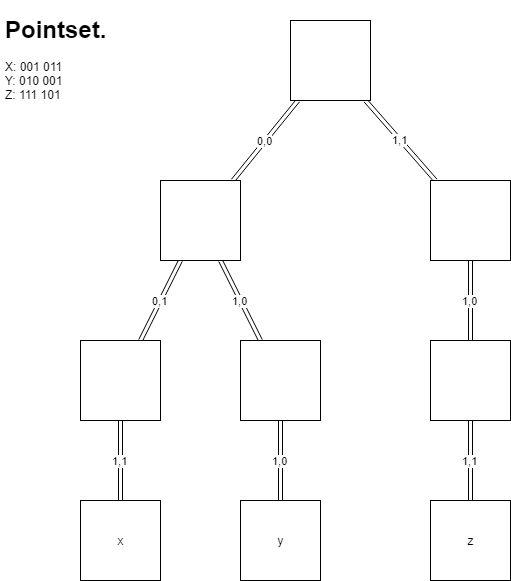
\includegraphics[width=0.5\textwidth]{figures/quadtree}
	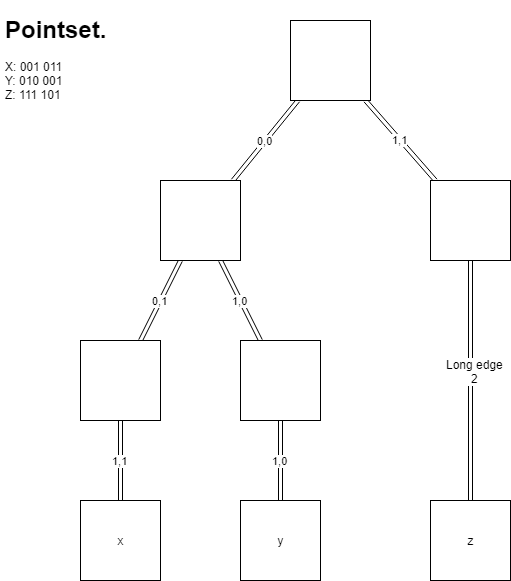
\includegraphics[width=0.5\textwidth]{figures/prunnedquadtree}
	\caption{On the left there is shown the \qt{} after construction with $L=4$. On the right the \qt{} has been pruned with a $\Lambda = 1$}
	\label{fig:quadtree}
\end{figure}

The final step is the pruning. For each downward path $n_0,...,n_k$ in the \qt{} where nodes $n_1,...,n_{k-1}$ all have a degree 1, if \ensuremath{\texttt{k} > \Lambda+1} then corresponding nodes $n_{\Lambda+1},...,n_{k-1}$ are removed from the \qt{}. Instead node $n_{\Lambda}$ is connected directly to $n_{k}$ with an edge. This edge is called a \textit{long edge} and is labeled with the length of the path it replaces. An example of the tree after a pruning is given in figure \ref{fig:quadtree}.


From the above briefly described steps the sketch is built. To represent the sketch the "Eulerian Tour Technique"\footnote{See e.g., \url{https://en.wikipedia.org/wiki/Euler\_tour\_technique}} is used.
It starts at the root of the tree and searches down to the leftmost leaf. It will then backtrack up to a node from which it can again traverse down to find a new leaf. When an edge is explored downwards there is stored a 0 and the label of the edge, being either a bit string or the length of a long edge. Also for each downward movement a bit specifying if the given edge is a long or short edge is stored. If an upwards edge is explored then a 1 is stored. Furthermore, there is stored for each point an index for the child node which contains it.
%TODO: Review this subsection to properly and precisely describe QS

%From ILO:
%"Find, extract and explain results in the algorithms research literature relevant to a given problem."
\subsection{Related work}
\label{state_of_the_art}
As the research area, described in \ref{research_area}, is as big as it is, a huge amount of related work to \qs{} exists. \cite{wagner17} specifically compares their algorithm to a state of the art algorithm, \textit{Product Quantization} (\pq{}), introduced in \cite{schmid9}. 

\subsubsection{\textit{Product Quantization}}
The \pq{} concept is stated in the abstract of the original paper as such: "This paper introduces a product quantization based approach for approximate nearest neighbor search[ANN]. The idea is to decompose[ ] the space into a Cartesian product of low dimensional subspaces and to quantize each subspace separately". Specifically the algorithm uses \textit{vector quantization} as the approach to compress data, mapping a real valued vector, \textit{x}, in \textit{D}-dimensional space to \textit{centroid} representations, \textit{$c_i$}, in a set $\mathcal{V}_i$\cite[p.3 II-A]{schmid9}. The set of vectors mapped with the quantizer function \textit{q} to a given index \textit{i} is referred to as a (Voronoi) \textit{cell}, and defined as:

\begin{equation}
	\mathcal{V}_i\mathrel{\hat=}{x\in\mathbb{R}^D : q(x)=c_i}
\end{equation}

As opposed to scalar quantization, where single values are reconstructed, in this case the set of \textit{vectors}, indexed to the same cell, are reconstructed. Before applying this scheme to the vectors, the D dimensions are divided into \textit{product quantizers}, basically dividing the space into \textit{m} subvectors of \textit{D*} dimensions, such that \textit{D*$=D/m$}\cite[p.3 II-B]{schmid9}. The subvectors are then quantized seperately using \textit{m} distinct quantizers. This scheme is applied, allowing to keep very large vector codes in memory. As reference a convincing example is listed in \cite[Table I, p. 4]{schmid9}, illustrating that the k-means algorithm consumes $kD$ memory, while k-means with product quantization consumes  $k^{1/m}D$.

Besides using \pq{} as comparison algorithm in their experiments, \qs{} is actually implemented\footnote{specifically defined in \tm{3}, \cite[p. 5]{wagner17}} with the same idea of \textit{product quantizers}..

\subsubsection{Spectral hashing}
%TODO: Relate
%TODO: More related work than 2?

\subsubsection{Stefan}

%Well known general algorithms and data structures exists for the same purpose, such as \textit{k-means} and \textit{kd-trees}, where the former is a clustering algorithm and the latter is an adaptive data structure for spatial data sets. This is also discussed in \cite{schmid9}, where it is noted that apparently a pure brute-force algorithm outperforms these in practice for high-dimensional data. Further algorithms listed in this paper include "spectral hashing"\cite{weiss8}, "Hamming embedding"\cite{jegou8}, and "FLANN"\cite{muja9}. These will not be investigated further, but are only mentioned for reference.
%TODO: Elaborate on closely related work and insert citations